%% ****** Start of file aiptemplate.tex ****** %
%%
%%   This file is part of the files in the distribution of AIP substyles for REVTeX4.
%%   Version 4.1 of 9 October 2009.
%%
%
% This is a template for producing documents for use with 
% the REVTEX 4.1 document class and the AIP substyles.
% 
% Copy this file to another name and then work on that file.
% That way, you always have this original template file to use.

%\documentclass[aip,graphicx]{revtex4-1}
%\documentclass[aip,reprint]{revtex4-1}

%\usepackage{graphicx}

%\draft % marks overfull lines with a black rule on the right
%\documentclass[pre,aps,floatfix,authordate1-4,twocolumn]{revtex4-1}
%\documentclass[pre,aps,floatfix,authordate1-4]{revtex4-1}

\documentclass[aps,prl,superscriptaddress,twocolumn]{revtex4}



%\documentclass[aps,prl,preprint,groupedaddress]{revtex4}

\usepackage{rotating} 
\usepackage{times}
\usepackage{graphicx}
\usepackage{setspace}
\usepackage{amsmath}
\usepackage{epstopdf}
\usepackage[obeyFinal]{easy-todo}
\usepackage{csquotes}
\usepackage{xr-hyper}
\usepackage{hyperref} % to make TOC titles clickable
\hypersetup{
    colorlinks=true, %set true if you want colored links
    linktoc=all,     %set to all if you want both sections and subsections linked
    linkcolor=black,  %choose some color if you want links to stand out
    citecolor=black,
    filecolor=black,
    urlcolor=black
}

\makeatletter
\newcommand*{\addFileDependency}[1]{% argument=file name and extension
  \typeout{(#1)}
  \@addtofilelist{#1}
  \IfFileExists{#1}{}{\typeout{No file #1.}}
}
\makeatother

\newcommand*{\myexternaldocument}[1]{%
    \externaldocument{#1}%
    \addFileDependency{#1.tex}%
    \addFileDependency{#1.aux}%
}

\myexternaldocument{manuscriptPGPEsuppl}

\begin{document}

% Use the \preprint command to place your local institutional report number 
% on the title page in preprint mode.
% Multiple \preprint commands are allowed.
%\preprint{}

\title{NMRlipids IV: Headgroup \& glycerol backbone structures, and cation binding in bilayers with PE and PG lipids} %Title of paper

% repeat the \author .. \affiliation  etc. as needed
% \email, \thanks, \homepage, \altaffiliation all apply to the current author.
% Explanatory text should go in the []'s, 
% actual e-mail address or url should go in the {}'s for \email and \homepage.
% Please use the appropriate macro for the type of information

% \affiliation command applies to all authors since the last \affiliation command. 
% The \affiliation command should follow the other information.

\author{Am{\'e}lie Bacle}
\affiliation{Laboratoire Coopératif "Lipotoxicity and Channelopathies – ConicMeds", Université de Poitiers, 1 rue Georges Bonnet, 86000 Poitiers, Franc }

\author{Pavel Buslaev}
\affiliation{Nanoscience Center and Department of Chemistry, University of Jyväskylä, P.O. Box 35, 40014 Jyväskylä, Finland}
\affiliation{Research Center for Molecular Mechanisms of Aging and Age-related Diseases, Moscow Institute of Physics and Technology, 141701 Dolgoprudny, Russia}

\author{Rebeca Garc{\'i}a Fandi{\~n}o}
\affiliation{Center for Research in Biological Chemistry and Molecular Materials (CiQUS), Universidade de Santiago de Compostela, E-15782 Santiago de Compostela, Spain}
\affiliation{CIQUP, Centro de Investigação em Química, Departamento de Química e Bioquímica, Faculdade de Ciências, Universidade do Porto, Porto, Portugal}

\author{Fernando Favela-Rosales}
\affiliation{Departamento de Ciencias B\'{a}sicas, Tecnol\'{o}gico Nacional de M\'{e}xico - ITS Zacatecas Occidente, M\'{e}xico}

\author{Tiago M. Ferreira}
\affiliation{NMR group - Institute for Physics, Martin Luther University Halle-Wittenberg, 06120 Halle (Saale), Germany}

\author{Patrick F.J. Fuchs}
\affiliation{Sorbonne Université, Ecole Normale Supérieure, PSL University, CNRS, Laboratoire des Biomolécules (LBM), 75005 Paris, France}
\affiliation{Université de Paris, UFR Sciences du Vivant, 75013, Paris, France}

\author{Ivan Gushchin}
\affiliation{Research Center for Molecular Mechanisms of Aging and Age-related Diseases, Moscow Institute of Physics and Technology, 141701 Dolgoprudny, Russia}

\author{Matti Javanainen}
\affiliation{Institute of Organic Chemistry and Biochemistry of the 
Czech Academy of Sciences, Flemingovo n\'{a}m. 542/2, CZ-16610 Prague 6, Czech Republic}

\author{Anne M. Kiirikki}
\affiliation{Institute of Biotechnology, University of Helsinki}


\author{Jesper J. Madsen}
\affiliation{Department of Chemistry, The University of Chicago, Chicago, Illinois, United States of America}
\affiliation{Global and Planetary Health, College of Public Health, University of South Florida, Tampa, Florida, United States of America}

\author{Josef Melcr}
\affiliation{Institute of Organic Chemistry and Biochemistry of the 
Czech Academy of Sciences, Flemingovo n\'{a}m. 542/2, CZ-16610 Prague 6, Czech Republic}
\affiliation{Groningen Biomolecular Sciences and Biotechnology Institute 
and The Zernike Institute for Advanced Materials, 
University of Groningen, 9747 AG Groningen, The Netherlands}

\author{Paula Milan Rodriguez}
\affiliation{Sorbonne Université, Ecole Normale Supérieure, PSL University, CNRS, Laboratoire des Biomolécules (LBM), 75005 Paris, France}

\author{Markus S. Miettinen}
% \affiliation[Max Planck Institute of Colloids and Interfaces]{Department of Theory and Bio-Systems, Max Planck Institute of Colloids and Interfaces, 14424 Potsdam, Germany}
\affiliation{Department of Theory and Bio-Systems, Max Planck Institute of Colloids and Interfaces, 14424 Potsdam, Germany}

\author{O. H. Samuli Ollila}
\email[]{samuli.ollila@helsinki.fi}
\affiliation{Institute of Biotechnology, University of Helsinki}

\author{Chris G. Papadopoulos}
\affiliation{Université Paris-Saclay, CEA, CNRS, Institute for Integrative Biology of the Cell (I2BC), 91198 Gif-sur-Yvette, France}


\author{Antonio Pe{\'o}n}
\affiliation{Spain}

\author{Thomas J. Piggot}
\affiliation{Chemistry, University of Southampton, Highfield, Southampton SO17 1BJ, United Kingdom}

\author{{\'A}ngel Pi{\~n}eiro}
\affiliation{Departamento de F{\'i}sica Aplicada, Facultade de F{\'i}sica, Universidade de Santiago de Compostela, E-15782 Santiago de Compostela, Spain}


% Collaboration name, if desired (requires use of superscriptaddress option in \documentclass). 
% \noaffiliation is required (may also be used with the \author command).
%\collaboration{}
%\noaffiliation

\date{\today}

\begin{abstract}
% insert abstract here
  Chemistry of lipid headgroups, the water facing components of cell membranes that regulate cell functions via lipid--protein interactions, varies between organisms and organelles. Because membranes are in liquid state under physiological conditions,
  individual lipids are not fixed to single conformations but they sample an ensemble of conformations with the Boltzmann weighted probabilities.
  However, these ensembles and their dependence on lipid types have not yet been experimentally determined. 
  Therefore, it has not been clear if lipid molecules exchange between few rigid conformations,
  or if they can freely fluctuate in all possible conformations.
  Here, we combine solid state NMR experiments and molecular dynamics simulations from the NMRlipids open collaboration to resolve the conformational ensembles of the headgroups of key lipid types in their liquid lamellar phase under various biologically relevant conditions. Interpretation of NMR experiments using the plethora of simulation data collected in the NMRlipids project suggests that all lipid headgroups sample a wide range of conformations in neutral and charged cellular membranes.
  Differences in the headgroup chemistry between different lipid types manifest
  in probability distributions of conformations, but all lipid types can access almost any of the possible conformations.
  Together with the analysis of protein-bound lipids from the protein data bank (PDB), this suggests that lipids can bind to proteins in a wide range of conformations independently of their headgroup chemistry. Therefore, the selective adsorption of proteins to membranes is likely regulated by specific protein--lipid interactions rather than conformational restrictions of the bilayer lipids.
  Our results pave the way to comprehensive understanding of
  lipid mediated signaling and lipid--protein interactions in biomedical applications.

  
\end{abstract}

%\pacs{}% insert suggested PACS numbers in braces on next line

\maketitle %\maketitle must follow title, authors, abstract and \pacs

% Body of paper goes here. Use proper sectioning commands. 
% References should be done using the \cite, \ref, and \label commands


%\label{}
\section{Introduction}

Chemical compositions of hydrophilic lipid headgroups vary between different
organelles and organisms, and different lipid types
regulate protein functions in many different ways \cite{lee03,vanmeer08}.
Lipids can directly bind to proteins or indirectly affect protein
functions by altering membrane properties such as charge or elasticity \cite{lee03,lemmon08}.
Specific interactions with certain lipid headgroups
are known to be essential for the function of several proteins \cite{lee11,lemmon08},
but it is not clear if the specificity is driven by the
differences in accessible conformations between lipid types or
by specific lipid--protein interactions.

Stuctures of protein-bound lipids are available in the protein data bank (PDB) \cite{berman00}
and crystal structures of lipids have been determined \cite{buldt81,pascher92},
but their relation to the conformational ensembles in bulk membranes in the liquid lamellar phase remains unclear \cite{marsh13b}.
%In addition to the changes in lipid conformational ensembles upon binding to proteins,
%also the experimentally measured response of lipid headgroup to membrane bound charges remains poorly understood 
%due to the lack of suitable models to interpret the lipid conformational ensembles in liquid lamellar state \cite{Semchyschyn04}.
Most accurate experimental information on conformational ensembles of lipids
%in the physiologically relevant
in liquid lamellar phase are typically derived from NMR experiments, particularly from 
C--H bond order parameters measured using $^2$H NMR~\cite{seelig77c,davis83,Semchyschyn04}.
According to these experiments, the glycerol backbone conformations are largely similar irrespectively of the headgroup \cite{gally81} and
the headgroup conformations are similar in phosphatidylcholine (PC), phosphatidylethanolamine (PE) and phosphatidylglycerol (PG) lipids,
whereas the headgroup of phosphatidylserine (PS) lipids is more rigid \cite{wohlgemuth80,buldt81}. 
However, order parameter signs are not accessible in $^2$H NMR experiments \cite{ollila16}
and universal models to map order parameters to structural ensembles are not available \cite{pezeshkian18,akutsu20}.
Therefore, it is not clear if the conformational ensemble of lipid headgroups in liquid lamellar bilayer
is composed of exchange between few restricted conformations, or if lipid headgroups can fluctuate freely across a wide range of conformations.



Here, we use natural abundance $^{13}$C NMR experiments %(enabling the determination of order parameter signs)
and MD simulations from the NMRlipids open collaboration
to resolve the differences in the conformational ensembles between PC, PE, PG and PS lipid headgroups.
We elucidate also the effect of charges and protein binding to lipid headgroup conformations.
Zwitterionic PC and PE are the most common lipids in eukaryotes and bacteria, respectively \cite{vanmeer08,sohlenkamp16}.
PE is also the second most abundant glycerophospholipid in eukaryotic cells
and has been related to various diseases \cite{vance15,calzada16,patel17}.
PS and PG are the most common negatively charged lipids in eukaryotes and bacteria, respectively,
and their presence affect membrane protein functionality and signaling \cite{lemmon08,leventis10,sohlenkamp16,hariharan18}.
All the studied lipids specifically bind to various proteins \cite{yeagle14}.
%We use our results to elucidate also lipid--protein interactions and the effect of charges on lipid conformations.

Similarity of glycerol backbone and headgroup order parameters in model membranes and bacteria \cite{gally81,scherer87,seelig90}
suggest that our results can be used to 
%the results from model systems could be used to
understand the biological role of lipid headgroups in lipid--protein interactions.
These interactions are crucial, for example, in lipid mediated signaling \cite{lemmon08} and
design of phoshoplipid-specific antibodies \cite{vigant15}. 
%The lipid conformational ensembles in liquid lamellar state paves the way toward understanding the
%specific binding of different lipid types to membrane proteins and how they regulate the protein function.

%Notably, such measurements can be performed also on living cells \cite{gally81,scherer87,seelig90}.


\section{Methods}
\subsection{Experimental C--H bond order parameters}
The headgroup and glycerol backbone C--H bond order parameters of 1-palmitoyl-2-oleoyl-sn-glycero-3-phosphoethanolamine (POPE) and 1-palmitoyl-2-oleoyl-sn-glycero-3-phospho-(1'-rac-glycerol) (POPG), purchased from Avanti polar lipids, were measured using natural abundance $^{13}$C solid state NMR spectroscopy as described previously \cite{ferreira13,ferreira16}. The magnitudes of order parameters were determined from the chemical-shift resolved dipolar splittings using a R-type Proton Detected Local Field (R-PDLF) experiment~\cite{dvinskikh04}, and the signs from S-DROSS experiments~\cite{gross97} combined with SIMPSON simulations \cite{bak00}.
%The experiments were done in a Bruker Avance III 400 spectrometer operating at a $^1$H Larmor frequency of 400.03 MHz.
%Magic angle spinning (MAS) of the sample was used at a frequency of 5.15 kHz (R-PDLF experiment) and 5 kHz (S-DROSS experiment).
The NMR experiments were identical as in our previous work~\cite{antila19}. The POPE experiments were recorded at 310~K and POPG experiments at 298~K, where the bilayers are in the liquid disordered phase \cite{marsh13}.

Glycerol backbone peaks from both lipids, and the $\alpha$-carbon peak from POPE in the INEPT spectra 
were assigned based on previously measured POPC spectra~\cite{ferreira13}.
The $\beta$-carbon peak from POPE was assigned based on $^{13}$C chemical shift table for amines available
at \url{https://www.chem.wisc.edu/areas/reich/nmr/c13-data/cdata.htm}.
\todo{How were $\alpha$ and  $\gamma$-carbon peaks assigned in POPG?}.
The $\beta$-carbon peak from POPG overlapped with the g$_2$ peak from glycerol backbone
because their chemical environments are similar.
\todo{Details to be checked by Tiago}.

\subsection{Molecular dynamics simulations}

Molecular dynamics simulation data were collected and analyzed using
the methods from the NMRlipids Open Collaboration project (\url{nmrlipids.blogspot.fi}) \cite{botan15,catte16,ollila16,antila19}.
%\url{github.com/NMRlipids/NMRlipidsIVotherHGs}. 
Simulation details, accessibility information and quality evaluation of more than 70 systems simulated for this work are in the supplementary information.

Best models for the interpretation of lipid headgroup conformational ensembles from the experimental data were selected
using quality evaluation measures defined in the NMRlipids project.
Conformational ensembles of headgroup and glycerol backbone in PE and PG simulations were evaluated using the C--H bond order parameters \cite{botan15}. Interactions between different headgroups were evaluated by monitoring the changes in headgroup order parameters upon mixing the lipids \cite{antila19}. The ion binding affinities and response of lipids to bound charge were evaluated by monitoring the changes in lipid headgroup order parameters \cite{catte16,antila19}.

Relative energy costs for turning dihedral angles with respect to the most probable value (lowest energy) were estimated from the inverse Boltzmann formula $\Delta E(\theta) = -kT \left[\ln\left[p(\theta)\right]-\ln\left[p(\theta_0)\right] \right]$, where $p(\theta)$ is the dihedral angle distribution and $\theta_0$ is the most probable angle from MD simulation.


%\clearpage
\begin{figure*}[]
  \centering
%  \includegraphics[width=9.0cm]{../Figs/lipids.pdf}
  %  \includegraphics[width=9.0cm]{../Figs/HGorderparametersPCPSPEPG.eps}
   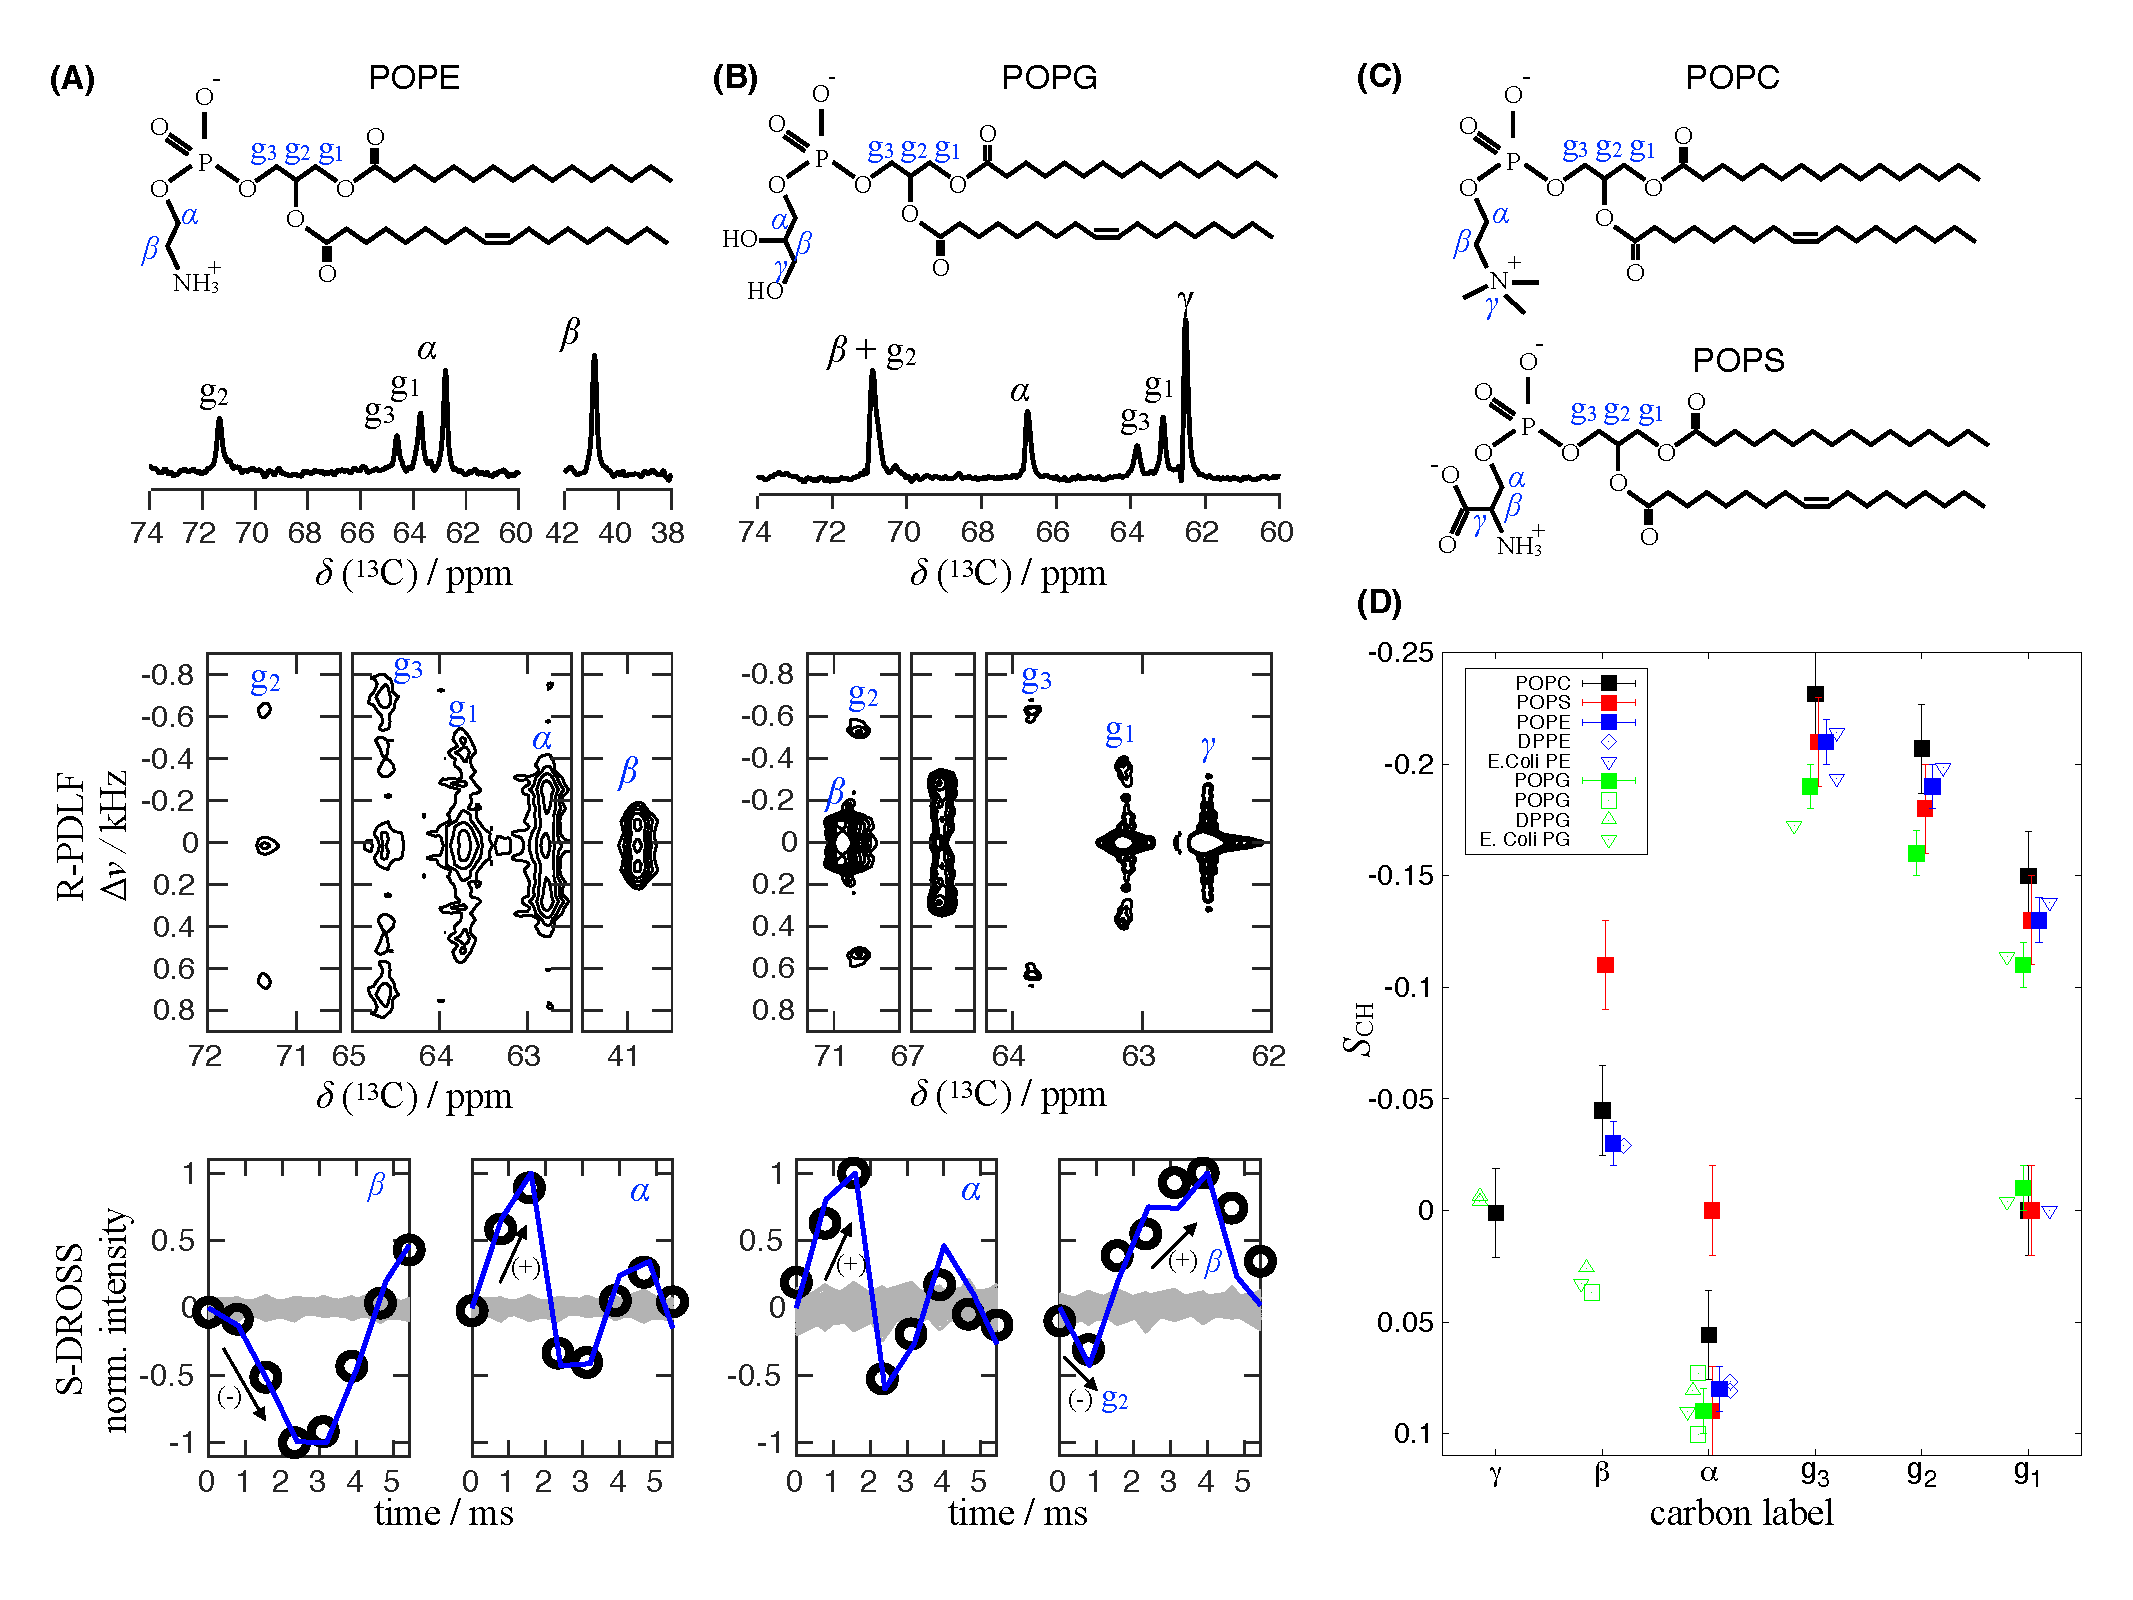
\includegraphics[width=18.0cm]{./Figs/figure1.pdf}
   \caption{\label{HGorderParameters}
     Chemical structure, refocused-INEPT spectrum, 2D R-PDLF spectra, and S-DROSS dipolar slices (from top to bottom) for \textbf{A)} POPE  and \textbf{B)} POPG MLVs measured by $^1$H-$^{13}$C solid-state NMR. The S-DROSS dipolar slices show both experimental data (open circles) and the result of NMR numerical simulations (blue solid lines).
      Full NMR spectra are shown in Figs. \ref{POPEspectra} and \ref{POPGspectra}.
     \textbf{C)} Chemical structure of POPC and POPS.
    \textbf{D)} Headgroup and glycerol backbone C-H bond order parameters for different phospholipids measured in the lamellar liquid disordered phase.
    The $S_{\rm{CH}}$ magnitudes and signs determined by $^1$H-$^{13}$C NMR spectroscopy (filled squares) for POPE (310~K) and POPG (298~K)
    measured in this work are shown together with the data previously reported for POPS (298~K) \cite{antila19} and POPC (300~K) \cite{ferreira13,ferreira16}. The headgroup and glycerol backbone $S_{\rm{CH}}$ magnitudes measured previously with $^2$H NMR (empty symbols) are also plotted as real values using the signs determined in this work for 
    POPG with 10nM PIPES (298~K) \cite{borle85},
    DPPG with 10mM PIPES and 100mM NaCl (314~K) \cite{wohlgemuth80}, 
    DPPE (341~K) \cite{seelig76},
    E.coli PE and E.coli PG (310~K) \cite{gally81}
    .
   }
   %\todo{This is a sketch, Tiago Ferreira will make a new figure.} \\
%  \todo{D) could be clarified as Fig. 2 in the NMRlipids IVps paper.}
\end{figure*}


\subsection{Analysis of protein-bound lipid conformations}
Lipid structures from the Protein Data Bank (PDB, \cite{berman2000})
were searched using PDBe REST API (\url{www.ebi.ac.uk/pdbe/pdbe-rest-api})
using the ligand names listed in the supplementary information.
Heavy atom dihedral distributions from the lipid structures were calculated
using the MDAnalysis Python library \cite{agrawal11,gowers16} and
Jupyter notebook available from \url{https://github.com/pbuslaev/scr/blob/master/PDB%20analysis.ipynb}.
Only the structures determined using X-ray crystallography or Cryo-EM with a resolution higher than 3.2~\text{\AA} were used in the analysis. Some structures of multimeric proteins contained multiple lipids in the same conformation (analyzed dihedral angles within 3 degrees of each other). In that case, this conformation was counted once for the subsequent analyses
to avoid its overweighting.
  
To demonstrate the existence of similar structures of different lipids bound to different proteins,
we searched for pairs having the last five dihedral angles (excluding g$_1$-g$_2$-g$_3$-O$_{g3}$) within
30 degrees of each other among the structures with resolution higher than 2.5~\text{\AA}. The two most representative examples
were handpicked from the results.


\section{Results and Discussion}

\begin{figure*}[bt]
  \centering
   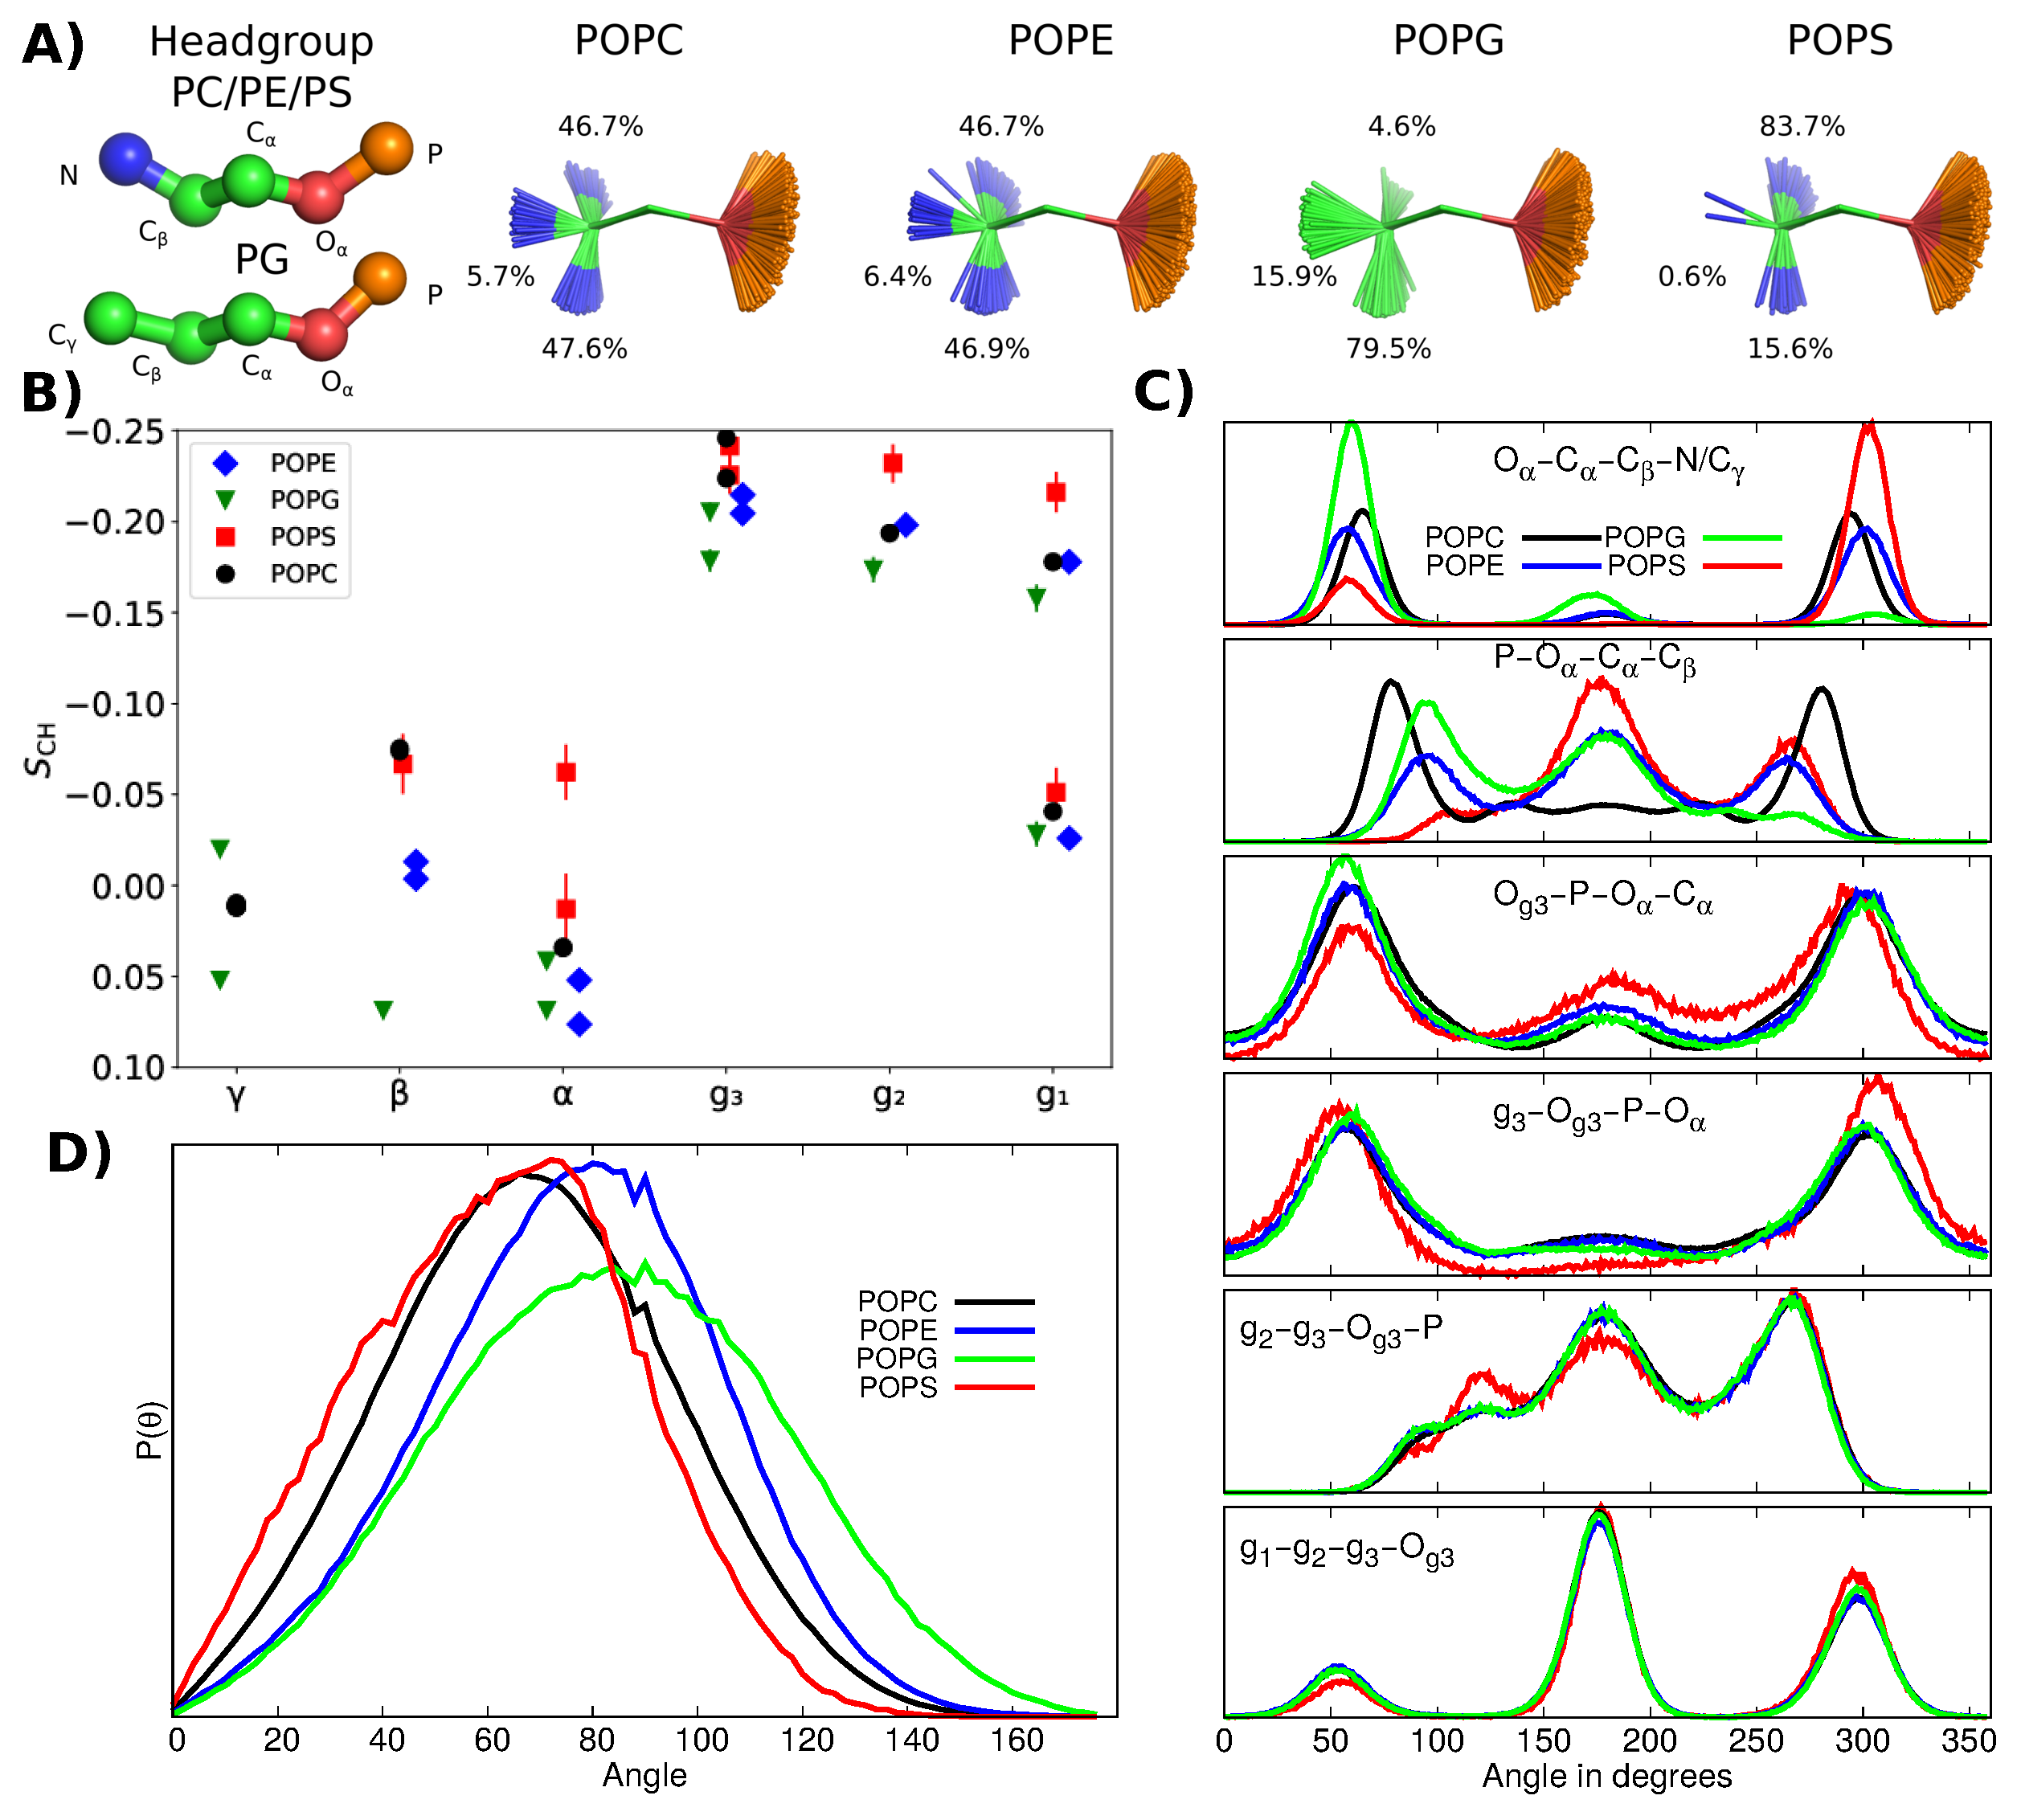
\includegraphics[width=18.0cm]{./Figs/figure2.eps}
   \caption{\label{structures}
     Results from the best simulation model (CHARMM36) simulations demonstrating the differences in conformational ensembles between different lipids. 
     \textbf{A)} Snapshots with overlayed C$_\beta$, C$_\alpha$ and O$_\alpha$ atoms and occurence of different conformations.
     \textbf{B)} Headgroup and glycerol backbone region order parameters of different different lipids.
     \textbf{C)} Relative free energies for individual heavy atom dihedral angles estimated from the inverse Boltzmann formula.
     Angles corresponding energies above 7~$k\mathrm{B}T$ are not shown because they are not observed in simulations.
     \textbf{D)} Distributions of P--N vector angle with respect to membrane normal.
  }
\end{figure*}


\subsection{Differences between lipid headgroups from $^{13}$C NMR experiments}

To experimentally characterize the differences in headgroup conformational ensembles of lipids that are not
bound to proteins in an electrostatically neutral cell membrane, we measured the C--H bond order parameters
and their signs of POPG and POPE in the liquid lamellar phase, as we did previously for POPC and POPS \cite{ferreira13,ferreira16,antila19}.
Determination of headgroup and glycerol backbone order parameters and their signs
was straightforward from the data in Figs.~\ref{HGorderParameters}, \ref{POPEspectra} and \ref{POPGspectra}
for all the C--H bonds, except for the $\beta$ and g$_2$ carbons in POPG.
These carbons have overlapping peaks in the INEPT spectra due to their similar chemical environments,
and only the magnitude of the larger order parameter could be determined from the R-PDLF spectra (Fig.~\ref{HGorderParameters}B).
Based on previous $^2$H NMR measurements \cite{wohlgemuth80,gally81,borle85},
we assigned the larger order parameter to the g$_2$ carbon
and used the literature value for the $\beta$-carbon in SIMPSON simulations to determine the signs.
The decrease in the beginning of the S-DROSS curve suggests that the sign of larger g$_2$ order parameter
is negative and later increase suggests that sign of smaller $\beta$ order parameter is positive (Fig.~\ref{HGorderParameters}B).
This interpretation is confirmed by SIMPSON calculations in Fig.~\ref{POPGsimpson}.

Experimental order parameters of POPC, POPE, POPG and POPS glycerol backbones and headgroups from this and previous studies are collected in Fig.~\ref{HGorderParameters}D, where signs determined from $^{13}$C NMR experiments are used also for the $^2$H NMR data from the literature. The overall agreement of order parameters determined by different research teams and different techniques for the same lipid headgroup is excellent here and in previous studies \cite{botan15,ollila16,antila19}. Therefore, the differences between lipid types are dictated by the headgroup chemistry rather than inaccuracies in experiments, differences in the acyl chains, or in experimental conditions.


The most distinct order parameters are observed for PS headgroups, for which the $\alpha$-carbon order parameter exhibits significant forking (different values for different hydrogens bound to the same carbon) and the $\beta$-carbon has a more negative value than other studied lipid types. On the other hand, the $\beta$-carbon order parameter of PG headgroup has a positive sign, in contrast to all the other lipid types. This has not been previously observed  in $^2$H NMR experiments detecting only the absolute values~\cite{wohlgemuth80,gally81,borle85}. The glycerol backbone order parameters are similar for all the lipid types, although they move slightly toward positive values (closer to zero) in the order PC $<$ PE $<$ PS $<$ PG. Only minor differences between PC and PE headgroups are observed.

\subsection{Conformational ensembles of different lipid headgroups from MD simulations}

\begin{figure*}[bt]
  \centering
  \includegraphics[width=18.0cm]{./Figs/HGorderparametersPCvsSURFchangeDIHEDRALSlog.eps}
  \caption{\label{changesWITHsurf}
    \textbf{A)} Modulation of PC headgroup order parameters and P--N vector angle upon addition of cationic surfactant (dihexadecyldimethylammonium)
    from CHARMM36 simulations compared with the experimental data \cite{scherer89}.
    \textbf{B)} Relative energies for individual dihedral angles estimated from inverse Boltzmann distributions of heavy atom dihedral angles
    with different amounts of cationic surfactant from CHARMM36 simulations.
  }
\end{figure*}

To understand the structural origin of distinct order parameters for PG and PS lipids,
we first calculated the heavy atom dihedral angle distributions from simulations
that best reproduce the differences between headgroups according to the quality
evaluation in the SI and Refs. \cite{botan15,antila19} (Fig. \ref{DIHdists}).
Then, we used the inverse Boltzmann formula to estimate the
energy costs for different dihedral angle orientations.
The results in Fig.~\ref{structures}C suggest that all lipid headgroups are very flexible and
energy costs for rotating individual dihedrals to almost any angle is low (below 7~$k_\mathrm{B}T$).
Only $cis$ states of P-O$_\alpha$-C$_\alpha$-C$_\beta$ and g$_2$-g$_3$-O$_{g_3}$-P have larger relative
energies and are not observed for any lipids during the simulations.


Major differences between headgroups are observed for the last two dihedrals in the headgroup end,
O$_\alpha$-C$_\alpha$-C$_\beta$-N/C$_\gamma$ and P-O$_\alpha$-C$_\alpha$-C$_\beta$,
which prefer \textit{gauche$^-$} conformations for PG and \textit{gauche$^+$} for PS,
whereas PC and PE exhibit symmetric distributions.
Also, the energy barriers for O$_\alpha$-C$_\alpha$-C$_\beta$-N/C$_\gamma$ dihedral
rotations between \textit{gauche} and \textit{trans} states are larger for
PS and PG lipids than for PC and PE lipids. 
Rest of the dihedrals are similar between different lipids,
with the exception of PS lipids for which slightly larger energy for \textit{eclipsed anti} conformation
in g$_3$-O$_{{\mathrm g}3}$-P-O$_\alpha$ dihedral was observed.
Therefore we suggest that the main differences between lipid headgroups leading to distinct order parameters occur in the choline part, while also changes in phosphate region may contribute in PS lipids. The increased barriers for dihedral rotations may explain the more rigid headgroup structures in PS~\cite{browning80,buldt81}. Furthermore, the angle between headgroup dipole and membrane normal decreases in the order of PG $>$ PE  $>$ PC  $>$ PS (Fig.~\ref{structures}D). However, the differences between PC and PE in P-O$_\alpha$-C$_\alpha$-C$_\beta$ dihedral
and P--N vector dipole may be artificial as the $\beta$-carbon order parameter in PC is too negative even in the best available force field, thereby not being equal to the order parameter in PE as observed in experiments \cite{botan15}.

In conclusion, all studied lipid headgroups sample very broad conformational ensembles in the liquid lamellar phase and the sampled dihedral angles are within approximately same ranges for all headgroup types. % (Fig. \ref{structures}).
Since the rotation of dihedral angles to almost any position bears relatively low free energy cost,
%results suggest that all lipid headgroups are very flexible---
%thereby being
the lipid headgroups are able to adopt a wide range of conformations when interacting with proteins, ions, or other biomolecules.
%Our results support the models proposing free rotation around phosphate group for PC lipids, which decouples the dynamics and conformations between acyl chains and headgroups \cite{klauda08c,antila21b}, and suggests that these models could be applied for all lipids containing the phosphorus group.
%The wide range of observed conformations suggest that
Therefore, the structures in lipid crystals \cite{buldt81,pascher92} play only a minor role, and models aiming to explain NMR data using only a few conformations \cite{seelig77c,davis83,Semchyschyn04,akutsu20} are not sufficient to capture the large conformational space of lipids in the liquid lamellar state.



\subsection{Lipid conformational ensembles in charged membranes}

Charged entities, such as lipids, proteins, surfactants, drugs, and ions incorporated in membranes can reorient the headgroup dipole in PC lipids and affect the order parameters of the lipid headgroups \cite{seelig87}. However, the detailed understanding of the structural and energetic responses of lipids to membrane-bound electric charge is still lacking \cite{Semchyschyn04}.

To resolve lipid headgroup conformational ensembles in cell membranes bearing positive charge,
we calculated the heavy atom dihedral angle distributions from 
the subset of simulations %(CHARMM36)
that correctly captured the experimentally measured decrease in PC headgroup order parameters upon addition of cationic surfactants into a bilayer (figure \ref{changesWITHsurf} A).
The dihedral angle distributions and relative energies
in figures \ref{HGorderparametersPCvsSURFdihedrals} and \ref{changesWITHsurf} B) reveal that the
addition of positive charge into a membrane 
decreases the abundance of \textit{trans} states in g$_2$-g$_3$-O$_{g_3}$-P and g$_3$-O$_{g_3}$-P-O$_\alpha$
dihedrals.
The choline region remains essentially unchanged and only minor changes are observed in other dihedrals even at a surfactant molar fraction of 0.47.

In addition, binding of ions to the membrane may affect the lipid headgroup conformational ensembles under physiological conditions.
The bound Ca$^{2+}$ ion to PC headgroup leads to similar decrease in trans state probability for g$_3$-O$_{g3}$-P-O$_\alpha$ dihedral
in the most realistic MD simulations models
as observed for cationic surfactants
(lipid17ecc and CHARMM36 in Figs.~\ref{DIHSwithCAlipid17eccPOPC}, \ref{DIHSwithCAcharmm36POPC} and Fig.~\ref{changesWITHCaClPG}).
The dihedral distributions of the PG headgroup are more sensitive to the bound ions in the most realistic simulations,
but upward tilting of the headgroup dipole upon the addition of CaCl$_2$ is weaker than in PC
(Lipid17 and Slipids in Figs.~\ref{changesWITHCaClPG},~\ref{DIHSwithCAslipidsPOPG} and \ref{DIHSwithCAlipid17POPG}).
However, the changes in PG lipid dihedrals upon the addition of CaCl$_2$ differ between the best models (Figs.~\ref{DIHSwithCAslipidsPOPG} and~\ref{DIHSwithCAlipid17POPG}), and none of the simulations captures the Ca$^{2+}$ ion binding affinity and conformational ensemble of PG lipids simultaneously. Moreover, experimental data to evaluate the response of $\alpha$-carbon order parameters to the added CaCl$_2$ in PG is not available.
Additionally, the headgroup conformational ensembles in mixtures of PC and charged (PG or PS) or zwitterionic (PE)
lipids could not be resolved with the currently available force fields and experimental data
(Figs.~\ref{HGorderparametersPCvsPEPG} and~\ref{HGorderparametersPGvsPCchange}, and Ref.~\cite{antila19,melcr20}).


%Despite the difficulties in simulations to capture the headgroup conformations in mixtures involving charged lipids,
In conclusion, the structural response of lipid headgroups to 
%experimentally observed changes in headgroup order parameters upon addition of
membrane-bound charges arise
%from relatively small changes in conformational ensembles. These changes eventuate
from mild changes in dihedral angle distributions, rather than restriction of lipids to
fixed conformations. Therefore, lipid headgroups sample a large space of different conformations
also in charged membranes, thereby retaining the capability to adopt multiple conformations when
interacting with proteins or other molecules.



\subsection{Protein-bound lipid conformations}

\begin{figure*}[]
  \centering
  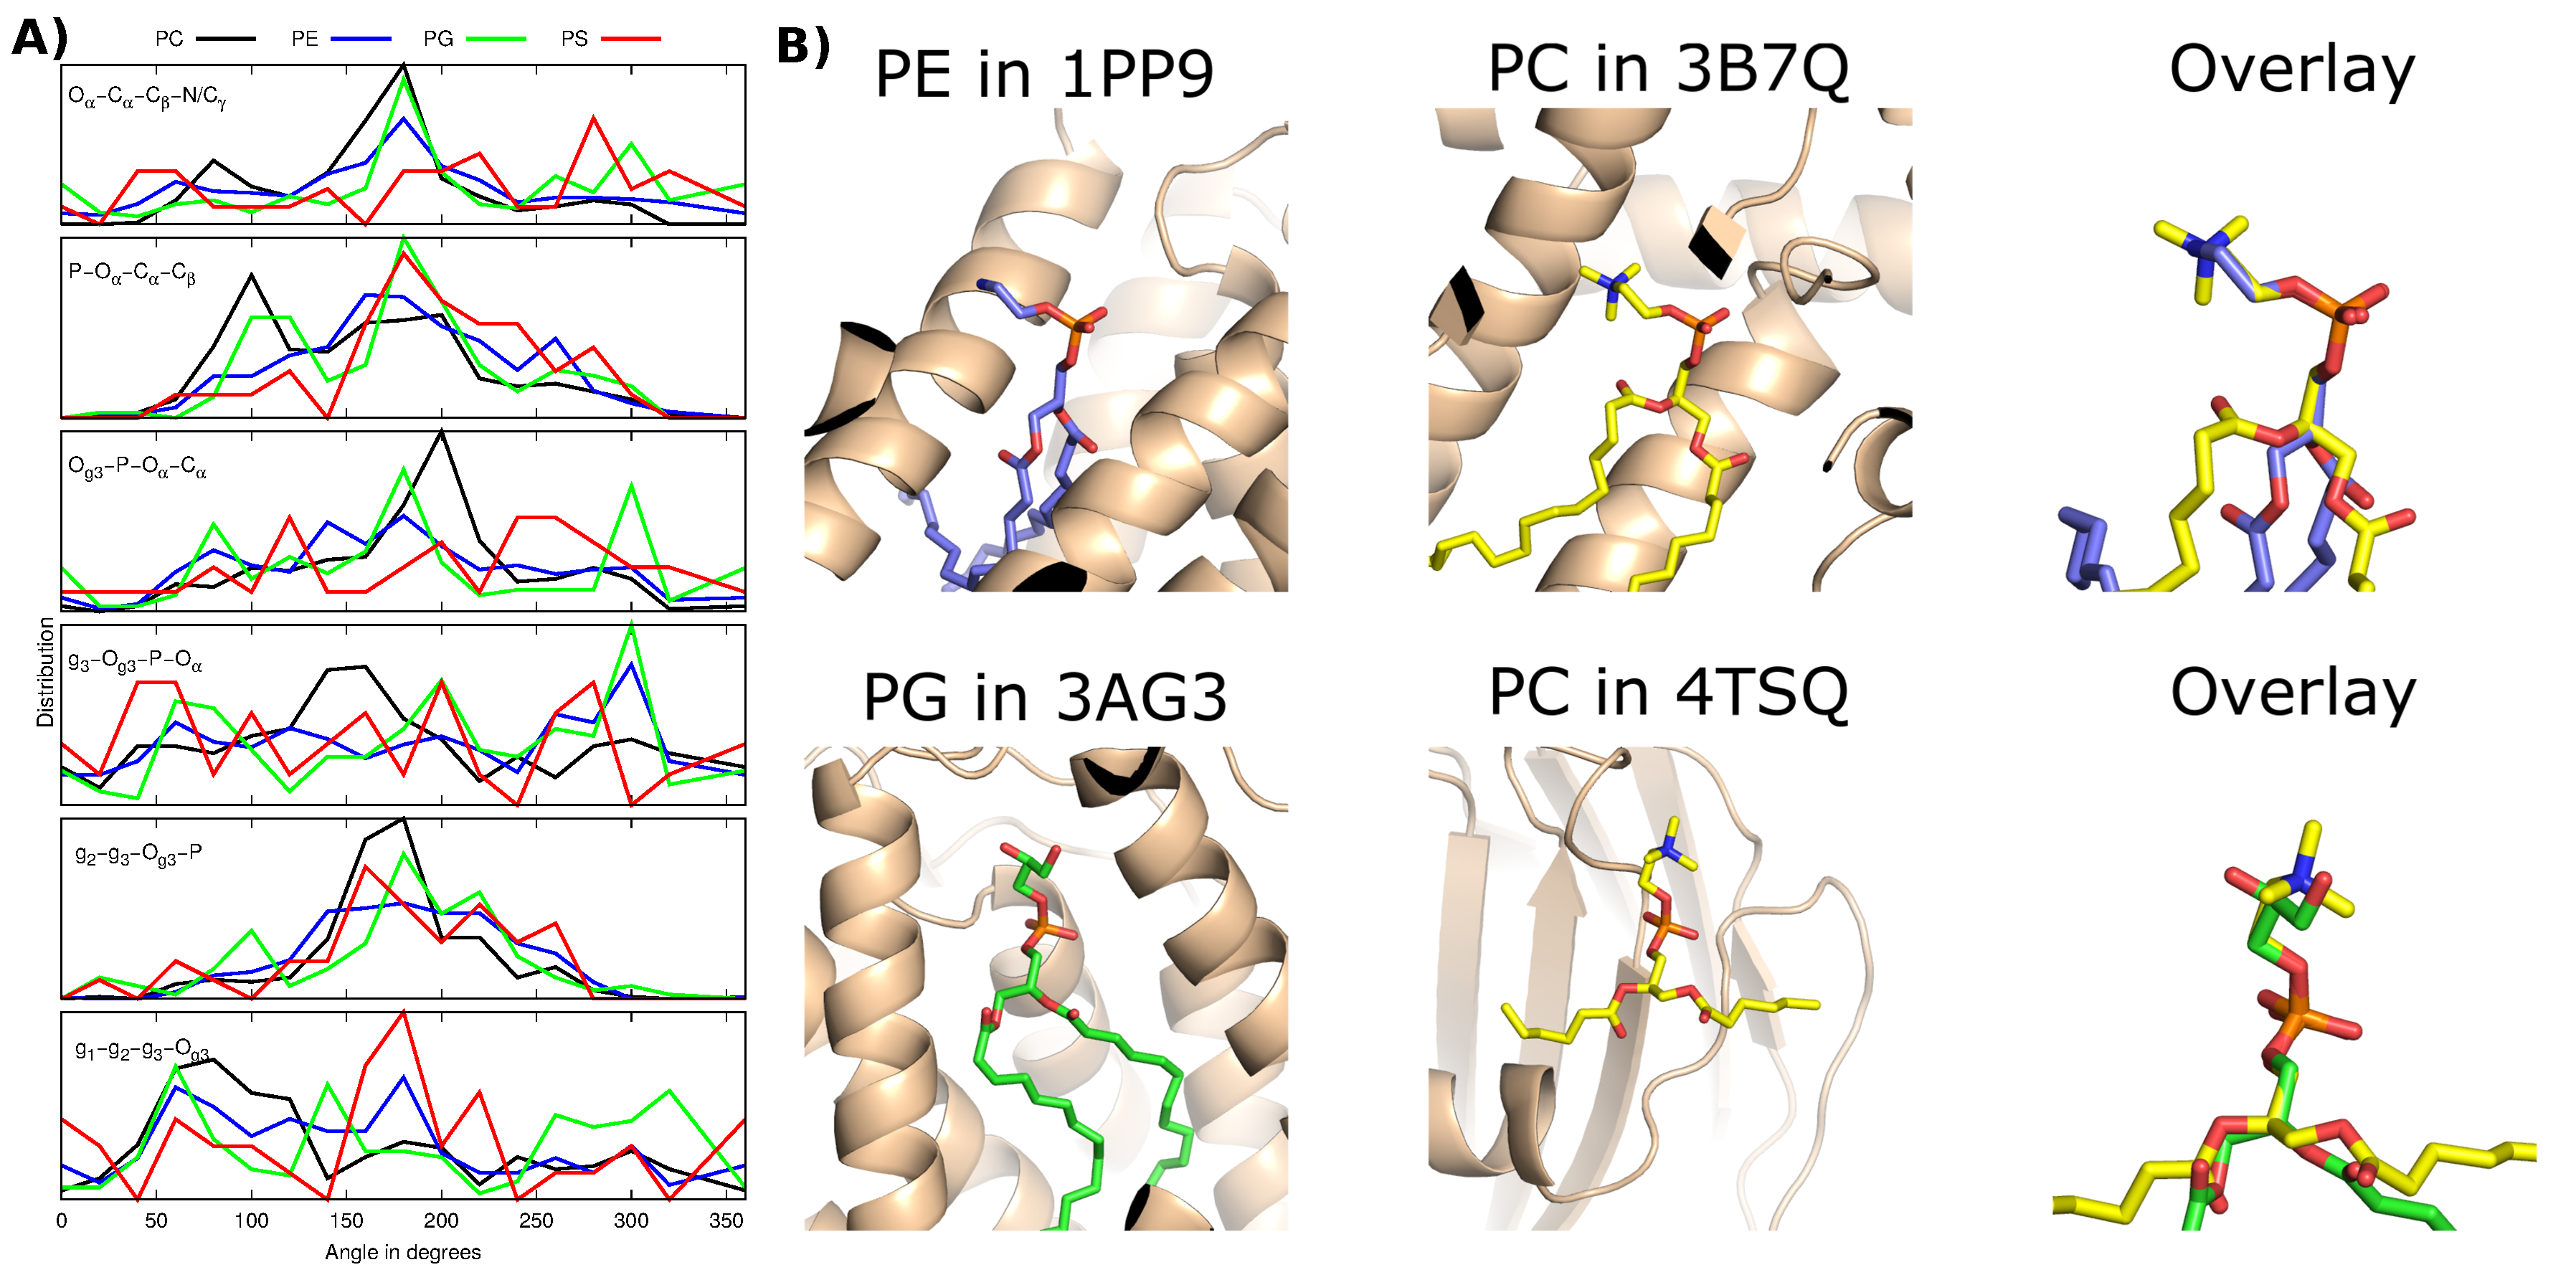
\includegraphics[width=19.0cm]{./Figs/figure4.eps}
  \caption{\label{dihedralsFROMpdb}
    A) Heavy atom dihedral angle distributions calculated from lipid structures in PDB.
    B) The structure of PE headgroup bound to cytochrome {\it bc}$_1$ complex (PDB ID: 1PP9 \cite{huang05})
    with identical conformation as the PC headgroup bound to yeast Sec14 (PDB ID: 3B7Q \cite{schaaf08}),
    and the structure of PG headgroup bound to bovine cytochrome {\it c} oxidase (PDB ID: 3AG3 \cite{muramoto10})
    with identical conformation as PC to FraC, a pore-forming toxin (PDB ID: 4TSQ \cite{tanaka15}).
  }
\end{figure*}


Interpretation of experimental order parameters using MD simulations
in previous sections suggest that PC, PE, PG and PS lipid headgroups are very flexible,
allowing them to bind proteins in various different conformations.
To test this prediction, we analyzed the protein-bound lipid conformations
from structures deposited in the PDB \cite{berman00}.
We found 311 PC, 394 PE, 154 PG, and 35 PS protein-bound lipid conformations
%presenting lipids that are tightly bound to proteins in fixed conformations
that were determined as a part of protein structure using crystallography or cryo-EM. 

The heavy atom dihedral angle distributions calculated from these conformations 
(Fig.~\ref{dihedralsFROMpdb} A) reveal that the protein-bound lipids indeed exhibit wide
range of conformations independently on the headgroup type.
As for bulk lipid bilayers, only $cis$ conformations
of P-O$_\alpha$-C$_\alpha$-C$_\beta$ and g$_2$-g$_3$-O$_{g_3}$-P dihedrals are almost
completely absent in all lipids, and significant differences between
different headgroups were not observed.
Structures deviating from lipid crystals 
have been previously proposed to indicate inaccuracies in lipid structures in PDB \cite{marsh13b,pezeshkian18}. 
However, we observe large deviations from lipid crystals structures also in conformational ensembles
that reproduce the NMR data in the liquid lamellar phase, indicating that such deviations
are realistic also in protein-bound states.
%The %range of available angles for
%O$_\alpha$-C$_\alpha$-C$_\beta$-N/C$_\gamma$ and
%g$_1$-g$_2$-g$_3$-O$_{g_3}$ dihedrals are even less restricted in protein bound state
%than in liquid lamellar phase where $cis$ and $anti$ eclipsed state were not present (Fig.~\ref{structures}). 
%Major differences between different lipid headgroups are not observed when bound to proteins.
%Slight preference for the trans state in O$_\alpha$-C$_\alpha$-C$_\beta$-/C$_\gamma$ dihedral of PC,
%and for positive angles in P-O$_\alpha$-C$_\alpha$-C$_\gamma$ dihedral of PS lipids with respect
%to other lipids could be present in the data, but the statistics is not sufficient for conclusions.
%Therefore, the differences in conformational ensembles between different
%lipids in liquid lamellar state in Fig.~\ref{structures} are not seen in the protein bound states.

Our results suggest that flexible lipid headgroups can optimize the intermolecular interactions with proteins by binding
in a wide range of conformations.
Therefore, the specific binding of lipids to proteins is not driven by the structural differences between headgroups.
This is demonstrated in Fig.~\ref{dihedralsFROMpdb} B with two examples where different lipids bound to
different proteins have almost identical headgroup conformations:
PE in cytochrome {\it bc}$_1$ complex is similar to PC bound to yeast Sec14,
and PG bound to bovine cytochrome {\it c} oxidase is similar to PC bound to pore-forming toxin (FraC).
On the other hand, a single lipid headgroup type is capable of accommodating various binding positions and as such would 
be able to specifically bind to many different kinds of binding sites in different proteins.

%However, it is important to note that lipids are often not the main target in
%structures deposited in PDB and therefore their conformations may be less reliable than those of proteins.


\section{Conclusions}

C--H bond order parameters from NMR experiments %in this and previous studies \cite{wohlgemuth80,buldt81,seelig87}
suggest that lipid headgroup conformational ensembles depend on lipid type (PC, PE, PG or PS) 
and accumulated membrane charge (cationic lipids, surfactants, ions or drugs). 
Our interpretation of these data, using MD simulations collected
within the NMRlipids open collaboration,
revealed that the differences in order parameters can be explained
by relatively small changes in dihedral angle probability distributions.
All studied headgroups (PC, PE, PG and PS) are flexible
and access a similar wide range of conformations with only very few restictions in dihedral orientations
also when charges are bound to membranes.
The observed differences in order parameters originate from
reweighting conformational probabilities rather than changes in accessible structures.

The flexibility and wide conformational space of headgroups suggest that protein--bound lipids can
adapt to various binding sites to optimize the intermolecular lipid--protein interactions.
We tested this prediction by analyzing the conformations of lipids that are tightly bound to proteins in from the PDB.
Indeed, also protein--bound lipids exhibit wide range of conformations without significant 
differences between different lipid types. Therefore, the specificify of lipid binding to proteins is not
regulated by accessible structures of lipids, and a single lipid type can adapt to various binding sites in proteins.

Our results pave the way toward the understanding of lipid-mediated cell signaling and how lipids regulate membrane protein function in general.
We suggest that the key to understand selective binding of certain lipid types to proteins
are intermolecular lipid--protein interactions, rather than conformational restrictions of the lipids.
On the other hand, broad conformational ensembles in bulk bilayers suggest that lipid crystal structures
play a minor role and that the entropic cost of lipid binding may be significant.
Finally, we demonstrated the power of open access MD simulation data from the NMRlipids open collaboration
to complement the data in the PDB for elucidating how complex systems made up of disordered biomolecules behave.



% If you have acknowledgments, this puts in the proper section head.
\begin{acknowledgments}
AP is grateful to the Centro de
Supercomputación de Galicia (CESGA) for use of the Finis
Terrae computer
%
MJ thanks CSC -- IT Center for Science for computational resources and the Emil Aaltonen foundation for financial support.s
    %     Put your acknowledgments here.

P.B. was supportedby the Academy of Finland (Grant 311031)

F.F.-R. acknowledges Tecnol\'{o}gico Nacional de M\'{e}xico Proyecto IT16C431, Direcci\'{o}n General de Asuntos del Personal Acad\'{e}mico (DGAPA) Programa de Apoyo a Proyectos de Investigaci\'{o}n e Innovaci\'{o}n Tecnol\’{o}gica (PAPIIT) IG100920, CONACyT Ciencia de Frontera 74884 for financial support and Miztli-Direcci\'{o}n de C\'{o}mputo y de Tecnolog\'{i}as de Informaci\'{o}n y Comunicaci\'{o}n (DGTIC) - Universidad Nacional Aut\'{o}noma de México (UNAM) (Project LANCAD-UNAM-DGTIC-057) facilities for computing-time allocation.

I.G. was supported by the Ministry of Science and Higher Education of the Russian Federation (agreement #075-00337-20-03, project FSMG-2020-0003). 

J.J.M. gratefully acknowledges financial support from the Carlsberg 
Foundation in the form of a postdoctoral fellowship while at 
the University of Chicago (grants CF15-0552, CF16-0639, and 
CF17-0783) and the research framework provided by the 
Research Computing Center at the University of Chicago.

\end{acknowledgments}


% Create the reference section using BibTe
\bibliography{refs.bib}

%\newpage
%\section{APPENDIX: The NMR results reported by Tiago Ferreira}

\listoftodos

\end{document}
%
% ****** End of file aiptemplate.tex ******
